\chapter{Изучение свободных затухающих электромагнитных колебаний}

\section{Цель работы}

Изучение основных характеристик свободных затухающих колебаний.

\section{Ход работы}

\begin{table}[h]
	\caption{}
	\begin{tabularx}{\textwidth}{|X|X|X|X|X|X|X|X|X|}
		\hline 
		$R_\text{м}$, Ом & T, мс & $2U_i$, дел & $2U_{i+n}$, дел & n & $\lambda$ & Q & R, Ом & L, мГн \\ 
		\hline 
		0 & 95  & 4.9  & 3.1  & 2 & 0.229 &  &  &  \\ 
		\hline 
		10 & 95  & 4.6 & 2.9 & 2 & 0.231 &  &  &  \\ 
		\hline 
		20 & 95 & 4.5  & 2.6  & 2  & 0.274 &  &  &  \\ 
		\hline 
		30 & 95  & 4.3 & 2.2 & 2 & 0.335 &  &  &  \\ 
		\hline 
		40 & 95 & 4.2 & 2.1 & 2  & 0.347  &  &  &  \\ 
		\hline 
		50 & 95 & 4.0 & 1.9 & 2 & 0.372  &  &  &  \\ 
		\hline 
		60 & 95 & 3.9 & 1.6 & 2 & 0.445 &  &  &  \\ 
		\hline 
		70 & 95 & 3.8 & 1.4 & 2 & 0.499 &  &  &  \\ 
		\hline 
		80 & 95 & 3.6 & 1.3 & 2 & 0.509 &  &  &  \\ 
		\hline 
		90 & 95 & 3.5 & 1.2 & 2 & 0.535  &  &  &  \\ 
		\hline 
		100 & 95 & 3.4 & 1 & 2 & 0.612 &  &  &  \\ 
		\hline 
		200 & 95 & 2.5 & 0.5 & 2  & 0.805 &  &  &  \\ 
		\hline 
		300 & 95 & 1.7 & 0.2 & 1 & 2.140 &  &  &  \\ 
		\hline 
		400 & 95 & 1.3 & 0.1 & 1 & 2.565 &  &  &  \\ 
		\hline 
	\end{tabularx} 
\end{table}

\[
\lambda=\frac{1}{n}\cdot \ln\frac{U_i}{U_{i+n}}
\]

$\lambda_1=\frac{1}{2}\cdot \ln\frac{4.9}{3.1}=0.22891654681274023$

$\lambda_2=\frac{1}{2}\cdot \ln\frac{4.6}{2.9}=0.23067278325131044$

$\lambda_3=\frac{1}{2}\cdot \ln\frac{4.5}{2.6}=0.2742829758744188$

$\lambda_4=\frac{1}{2}\cdot \ln\frac{4.3}{2.2}=0.3350788311676232$

$\lambda_5=\frac{1}{2}\cdot \ln\frac{4.2}{2.1}=0.34657359027997264$

$\lambda_6=\frac{1}{2}\cdot \ln\frac{4}{1.9}=0.3722202374737479$

$\lambda_7=\frac{1}{2}\cdot \ln\frac{3.9}{1.6}=0.4454864619449326$

$\lambda_8=\frac{1}{2}\cdot \ln\frac{3.8}{1.4}=0.4992644150555636$

$\lambda_9=\frac{1}{2}\cdot \ln\frac{3.6}{1.3}=0.5092847904972866$

$\lambda_10=\frac{1}{2}\cdot \ln\frac{3.5}{1.2}=0.5352207058507067$

$\lambda_11=\frac{1}{2}\cdot \ln\frac{3.4}{1}=0.6118877158110578$

$\lambda_12=\frac{1}{2}\cdot \ln\frac{2.5}{0.5}=0.8047189562170501$

$\lambda_13=\frac{1}{1}\cdot \ln\frac{1.7}{0.2}=2.1400661634962708$

$\lambda_14=\frac{1}{1}\cdot \ln\frac{1.3}{0.1}=2.5649493574615367$


\begin{figure}[h]
	\centering
	\caption{График зависимости $\lambda$ от $R_m$}
	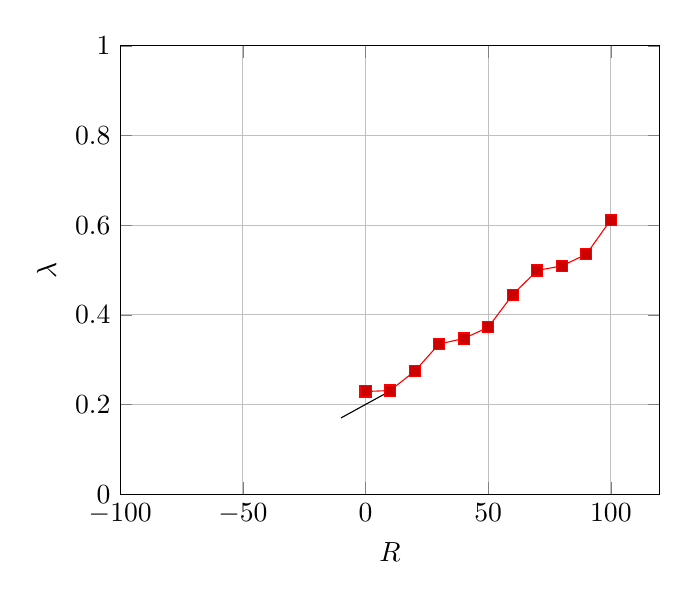
\begin{tikzpicture}
	\begin{axis}[
	xlabel=$R$,
	ylabel=$\lambda$,
	xmin=-100, xmax= 120,
	ymin=0, ymax=1,
	grid=major
	]
	\addplot[domain=-10:10, samples=100] {0.003*x + 0.2};
	\addplot coordinates {
		(0, 0.229)
		(10, 0.231)
		(20, 0.274)
		(30, 0.335)
		(40, 0.347)
		(50, 0.372)
		(60, 0.445)
		(70, 0.499)
		(80, 0.509)
		(90, 0.535)
		(100, 0.612)
	};
	\end{axis}
	\end{tikzpicture}
\end{figure}
